%Slide template developed by Mark E. Fuller from examples and miscellany produced at RWTH Aachen
%(probably mostly from the work of Philippe Dreuw and Thomas Deselaers)
%This template copyright Mark E. Fuller, 2021 (mark.e.fuller@gmx.de)

\documentclass[10pt,presentation]{beamer}

\usepackage[utf8]{inputenc}

%%%%%%%%%%%%%%%%%%%%%%%%%%%%%%%%%%%%%
%% Select language
%%
%\usepackage[ngerman]{babel}        % Deutsch, neue Rechtschreibung
%\usepackage[hebrew,english]{babel}  %example of declaring multilingual document; last listed is ``dominant''
\usepackage[english]{babel}

%regional add-ons
    % Shekel symbol
\DeclareRobustCommand{\ILS}{
\includegraphics[height=\fontcharht\font`T]{figures/ILS_bold}}

\DeclareRobustCommand{\ghinlinelogo}{
\includegraphics[height=\fontcharht\font`T]{figures/Logos/GitHub-Mark-120px-plus.png}}

\usetheme{custom}
\usepackage[T1]{fontenc}           % Font encoding (don't change!)
\usepackage{lmodern}               % Select Linux Modern Fonts (don't change)
\usepackage{sansmathfonts}         % Sans fonts in math environments
\usepackage{textcomp}              % fix 'missing font symbols' warning
\renewcommand{\rmdefault}{phv}     % Arial like (Helvetica)
\renewcommand{\sfdefault}{phv}     % Arial like (Helvetica)

%% graphics related packages
\usepackage{graphicx}              % needed to include graphics (don't change)
\usepackage{epstopdf}              % required to include eps files
%\usepackage{svg}                   % include svg files (requires Inkscape)
\usepackage{subfigure}             % option to layout figures in tabular environment
\usepackage[encoding,filenameencoding=utf8]{grffile} % allow utf8 file names in graphics´
\setbeamertemplate{caption}{\insertcaption} %no ``figure'' in caption
\usepackage{tikz}
\usepackage{curves}
\usepackage{pgfplots}
\usepackage{chemfig}
\setchemfig{angle increment=30, atom sep=2.75em}
%%%%%%%%%%%%%%%%%%%%%%%%%%%%%%%%%%%%%
%% import packages for content
%%
\usepackage{listings}              % display code: for lstlisting and \lstinline|..|

% mathematics
\usepackage{amsmath}
\usepackage{amssymb}
\usepackage{sansmath}

% tabularx -> better tabular environment
\usepackage{tabularx}
    % tabularx modifications
\newcolumntype{L}{>{\raggedright\let\newline\\\arraybackslash\hspace{0pt}}X}
\newcolumntype{R}{>{\raggedleft\let\newline\\\arraybackslash\hspace{0pt}}X}
\newcolumntype{C}{>{\centering\let\newline\\\arraybackslash\hspace{0pt}}X}
    % center text vertically in tabularx(column)
%\renewcommand{\tabularxcolumn}[1]{>{\large}m{#1}}

% Nicer tables
\usepackage{booktabs}
    % adjust table rows -> call on frame with table
\newcommand{\fixbooktabsrowhight}{%
    \setlength{\aboverulesep}{0pt}
    \setlength{\belowrulesep}{0pt}
    \setlength{\extrarowheight}{.5ex}
}
\usepackage{multirow} % cells with multiple rows
\usepackage{scrextend} %needed for footnotes in tables

% Source, e.g. for images
\setbeamercolor{framesource}{fg=gray}
\setbeamerfont{framesource}{size=\tiny}

\usepackage[absolute,overlay]{textpos}
\newcommand{\source}[1]{\begin{textblock*}{\linewidth}(1ex,\paperheight-2.75em)
        \begin{beamercolorbox}[left]{framesource}
            \usebeamerfont{framesource}\usebeamercolor[fg]{framesource} Source: {#1}
        \end{beamercolorbox}
\end{textblock*}}

\usepackage{etoolbox}
%% short titles for toc \(sub)section[SHORTTITLE for toc]{LONGTITLE for slide}
\makeatletter
% Insert [short title] for \section in ToC
\patchcmd{\beamer@section}{{#2}{\the\c@page}}{{#1}{\the\c@page}}{}{}
% Insert [short title] for \section in Navigation
\patchcmd{\beamer@section}{{\the\c@section}{\secname}}{{\the\c@section}{#1}}{}{}
% Insert [short title] for \subsection in ToC
\patchcmd{\beamer@subsection}{{#2}{\the\c@page}}{{#1}{\the\c@page}}{}{}
% Insert [short title] for \subsection  in Navigation
\patchcmd{\beamer@subsection}{{\the\c@subsection}{#2}}{{\the\c@subsection}{#1}}{}{}
\makeatother

%easily format to multiple columns
\usepackage{multicol}

%properly display chemical formulas and structures
    % Formula subscripts using \ce{}
\usepackage[version=3]{mhchem} 
    % structure drawing package
%\usepackage{chemfig}
%\setchemfig{chemfig style={line width=1.0pt}, atom sep=2em, angle increment=30, bond join=true, arrow style={line width=1.0pt}, lewis sep=0.3em}
%\pgfplotsset{compat=1.13}
    % define repeated abbreviations
\newcommand{\nox}{NO$_x$}


% Bibliography and citations

%get proper bib with numbered entries
%\setbeamertemplate{bibliography item}{\insertbiblabel}

%footnote citations - replace \cite with \footcite or \footfullcite
\usepackage[backend=biber, style=chem-acs]{biblatex} %, style=authoryear-comp
\addbibresource{references.bib}
\addbibresource{ownpubspres.bib}

%shrink citations
\setbeamerfont{footnote}{size=\tiny}

%bibliography/citation style
\setbeamertemplate{bibliography item}{\insertbiblabel}
\setbeamercolor{bibliography item}{fg=black}
\setbeamercolor*{bibliography entry author}{fg=black}


%some additional formatting
\newcommand{\red}[1]{\textcolor{red}{#1}} %easy red text
\usepackage{ulem}
\newcommand{\soutthick}[1]{%
	\renewcommand{\ULthickness}{1.6pt}%
	\sout{#1}%
	\renewcommand{\ULthickness}{.4pt}% Resetting to ulem default
}


%document header
\title[Chemistry free software toolchain]{An open-source toolchain from molecular vibrations to detailed combustion}
\subtitle{how (some) physical chemists and chemical engineers have escaped proprietary software}
%\titlegraphic{}
\author[Fuller \& Kaplan]{Mark E. Fuller, Ph.D. and Kfir Kaplan}
\email{fuller@fedoraproject.org} % optionally
\institute{LibrePlanet 2022}
%\webaddress{www.informatik.rwth-aachen.de/mentoring} % overrides www.rwth-aachen.de
\date[20 March 2022]{\today}
\subject{Libre Planet 2022}
\keywords{Technion, Latex Beamer, template}

%\logo{\vskip-2mm\includegraphics[width=45mm]{../common/figures/Logos/RWTH/PCFC.png}\hspace{-2mm}} % optionally


%%%%%%%%%%%%%%%%%%%%%%%%%%%%%%%%%%%%%
%% configure template behaviour
%%-------------------------------
%%   secstart -- style of section start
%%               selectable parameters:
%%                 sectitle:  only provides section title
%%                 sectoc:    display section table of contents
%%                 <empty>:   display nothing on section start
\secstart{sectitle}
% disable PDF navigation icons
\setbeamertemplate{navigation symbols}{}

\begin{document}

\begin{frame}{About Us}
Mark and Kfir are both active in developing and contributing to FOSS projects within the scientific community including \textsc{Cantera}, the \textsc{Reaction Mechanism Generator}, and the \textsc{Automatic Rate Calculator}.

\vspace{10pt}

Mark:
\begin{itemize}
 \item Ph.D. in chemical engineering
 \item Linux/FOSS user and contributor over 15+ years
 \item Research foci are combustion chemistry, batteries, fuel cells, and heat transfer
 \item Currently employed in DevOps
\end{itemize}

\vspace{10pt}

Kfir:
\begin{itemize}
 \item Fourth-year undergraduate student at the Technion in Biochemical Engineering
 \item Contributes to FOSS for over a year
 \item Conducts research at \url{dana.net.technion.ac.il}
\end{itemize}

\end{frame}

\section{Introduction}


\begin{frame}{Chemistry 101}

A few points require some chemistry terminology:

\vspace{0.5cm}

 \begin{itemize}
  
  \item Atoms:
  \begin{itemize}
  	\item Basic units of matter, composed of protons, neutrons, and electrons
  	\item Categorized as elements as a function of number of protons
  	\item Protons and neutrons form a nucleus about which electrons orbit
  	\item Electrically charged and form bonds through arrangements of electrons
  \end{itemize}
  
  \item Molecules:
  \begin{itemize}
    \item Also called ``(chemical) species''
  	\item Comprised of connected atoms
	\item Has internal movement (rotation, vibration)
	\item Structure matters: hexene (\ce{C6H12}) $\neq$ benzene (\ce{C6H12})
  \end{itemize}
  
  \vspace{10pt}
  
	\hspace{29mm}\scalebox{0.5}{\chemfig{C-[1]C-[11]C=C-[1]C-[11]C}} \hspace{3mm}$\neq$\hspace{3mm} \scalebox{0.5}{\chemfig{C**6(-C-C-C-C-C-)}}
  
%  \item State:
%  \begin{itemize}
%  	\item A "snapshot" of a molecule
%  	\item Varies by the coordination of the atoms and the energy
%  	\item Exists in 3D space
%  \end{itemize}

 \end{itemize}
 
\end{frame}


\begin{frame}{Chemistry 101}

Only a few more terms!

\vspace{12pt}
 \begin{itemize}

  \item Reaction:
  \begin{itemize}
  	\item A process that changes one or more molecules into others
  	\item Has reactants (inputs) and products (outputs), but processes are reversible
  	\item Has rate, which determines how fast the process occurs
  \end{itemize}
  
  \item Transition state:
  \begin{itemize}
  	\item The highest-energy species that is generated during the reaction
  	\item Is a "bottleneck" of the reaction - it controls the rate
  	\item Allows for calculations of the reaction rates
  \end{itemize}
  
  \item Mechanism:
  \begin{itemize}
  	\item Combinations (sets) of reactions and species
  	\item Allow for simulation the time evolution of a chemical system
  	\item Depends on external conditions (temperature, pressure, constraints)
  \end{itemize}

 \end{itemize}
 
\end{frame}


\begin{frame}{Computational chemistry:\\ an essential science}

Just a few examples:

\vspace{0.5cm}

 \begin{itemize}
  \item Alternative bio and manufactured fuels
  \item Batteries and fuel cells
  \item Drug and pharmaceutical manufacturing and degradation
  \item Proteins and organic molecules
  \item Refining and materials synthesis
 \end{itemize}
 
 \vspace{0.5cm}
 
 We are moving from postdictive to predictive computational capabilities\footfullcite{Green.2020}
 
\end{frame}

\begin{frame}{Toolchain overview:\\ macro to micro-scale}
``Complete'' simulation of a chemical reactor:

\vspace{0.5cm}

 \begin{itemize}
  \item Global/macroscopic: temperature, pressure, chemical composition (TPX)
  \item Reactor/condition-specific implementation of laws of thermodynamics, conservation equations
  \item Chemical reactions for all chemical species
  \item Thermodynamic properties for all chemical species
 \end{itemize}
\end{frame}

\begin{frame}{Toolchain overview:\\ computing and sourcing properties}
Various computational approaches:

\vspace{0.5cm}

 \begin{itemize}
  \item ``Guess'' new species and thermodynamic properties from tabulated rules
  \item Estimate reaction rates by analogy to other reactions
 \end{itemize}
 
 or
 
 \begin{itemize}
  \item Compute molecular structures (many different methods)
  \item Calculate thermodynamic properties and reaction rates
 \end{itemize}
 
 \vspace{0.5cm}
 
 \{Cheap and fast\} versus \{expensive and slow\},\\
 but we need both approaches to solve real problems
\end{frame}

\begin{frame}{Guessing Species and Reactions}

\vspace{-8mm}

    \begin{multicols}{2}
    \begin{itemize}
        \item Hydrogen abstractions
        \begin{itemize}
            \item \ce{RH} + \ce{NO2} $\rightleftharpoons$ \ce{R} + \ce{HONO}
            \item \ce{RH} + \ce{NO2} $\rightleftharpoons$ \ce{R} + \ce{HNO2}
            \item \ce{RH} + \ce{NO} $\rightleftharpoons$ \ce{R} + \ce{HNO}
        \end{itemize}
        \item Nitrite/Nitrate/Nitro-/Nitroso- Compounds
        \begin{itemize}
            \item \ce{RONO} $\rightleftharpoons$ \ce{RO} + \ce{NO}
            \item \ce{RONO2} $\rightleftharpoons$ \ce{RO} + \ce{NO2}
            \item \ce{RNO2} $\rightleftharpoons$ \ce{R} + \ce{NO2}
            \item \ce{RNO} $\rightleftharpoons$ \ce{R} + \ce{NO}
        \end{itemize}
        \item Isomerizations  
        \begin{itemize}
            \item \ce{RONO} $\rightleftharpoons$ \ce{RNO2}
        \end{itemize}
        \item \ce{HONO} elimination
        \begin{itemize}
            \item \ce{RONO} $\rightleftharpoons$ alkene + \ce{HONO}
        \end{itemize}
        \item \nox\ cycling
        \begin{itemize}
            \item \ce{RO2} + \ce{NO} $\rightleftharpoons$ \ce{RO} + \ce{NO2}
            \item \ce{R} + \ce{NO2} $\rightleftharpoons$ \ce{RO} + \ce{NO}
        \end{itemize}
    \end{itemize}
    
    \columnbreak
    
    \null \vfill
    \begin{figure}
        \centering
        \resizebox{\columnwidth}{!}{
            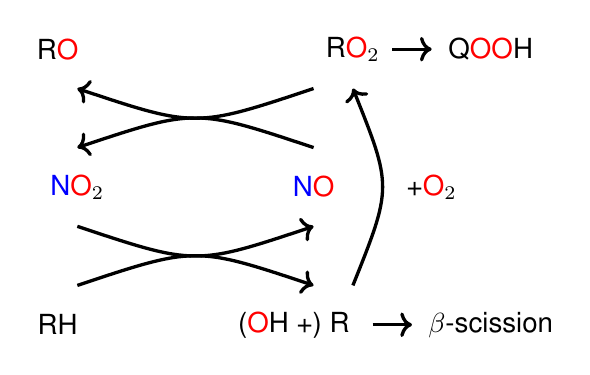
\begin{tikzpicture}
                %nox loop bounds
                \draw[->,very thick] (1,1) .. controls (2.5,0.5) .. (4,1);
                \draw[<-,very thick] (1,2) .. controls (2.5,2.5) .. (4,2);
                \draw (1,1.5) node {{\color{blue}N}{\color{red}O}$_2$};
                \draw (4,1.5) node {{\color{blue}N}{\color{red}O}};
                
                \draw[->,very thick] (1,0.25) .. controls (2.5,0.75) .. (4,0.25);
                \draw (0.75,-0.25) node {\ce{RH}};
                \draw (3.75,-0.25) node {({\color{red}O}H +) \ce{R} };
                
                \draw[<-,very thick] (1,2.75) .. controls (2.5,2.25) .. (4,2.75);
                \draw (0.75,3.25) node {R{\color{red}O}};
                \draw (4.5,3.25) node {R{\color{red}O}$_2$}; 
                
                \draw[->,very thick] (4.5,0.25) .. controls (5,1.5) .. (4.5,2.75); 
                \draw (5.5,1.5) node {+{\color{red}O}$_2$};
                
                \draw[->,very thick] (5,3.25)--(5.5,3.25); 
                \draw (6.25,3.25) node {Q{\color{red}O}{\color{red}O}H};
                
                \draw[->,very thick] (4.75,-0.25)--(5.25,-0.25); 
                \draw (6.25,-0.25) node {$\beta$-scission};
            \end{tikzpicture}
        }
        \label{fig:NOx_cycle}
        \caption{Adding \nox\ to a combustion process\footfullcite{Fuller.2021}}
    \end{figure}
    \vfill \null
    
    \end{multicols}
\end{frame}

\begin{frame}{Calculating Species and Reactions}

\vspace{-8mm}

	\begin{figure}
		\centering
        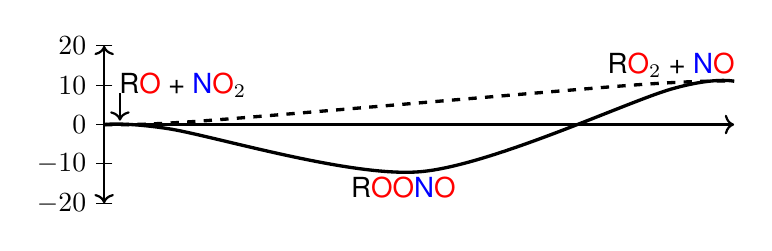
\begin{tikzpicture}[yscale = 0.5]
            %draw coordinate axis with labels
            %as above, not so many label, so they are manual here (e.g. make log)
            \draw[->,thick] (0,0) -- coordinate (x axis mid) (8,0);
            \draw[<->,thick] (0,2) -- coordinate (y axis mid)(0,-2);
            %\draw[gray, dashed](0,\ymax) grid (\Px,\ymin);
            \foreach \y/\ytext in {2/20, 1/10,0/0,-1/-10,-2/-20} \draw (3pt,\y cm) -- (-3pt,\y cm) node[anchor=east] {{$\ytext$}};
            
            %Text Labels
            %reactant side: placement will need to be adjusted for path lines
            \node [scale = 1.0,black] at (1.0, 1.0) {{R{\color{red}O} + {{\color{blue}N}{\color{red}O}$_2$}}};
            \node [scale = 1.0,black] at (7.2, 1.5){{R{\color{red}O}$_2$ + {{\color{blue}N}{\color{red}O}}}};      	
            \node [scale = 1.0,black] at (3.8, -1.60) {{R{\color{red}OO}{{\color{blue}N}{\color{red}O}}}};
            \draw[->,thick] (0.2,0.8) --(0.2,0.1);

            %links
            \draw[black, very thick] plot [smooth] coordinates {(0.0,0.0)(0.8,-0.1)(4.0, -1.2)(7.2,0.9)(8.0, 1.1)};
            \draw[black, very thick, dashed] plot [smooth] coordinates {(0.0,0.0)(1.3,0.1)(6.7,1.0)(8.0, 1.1)};
        \end{tikzpicture}
		\caption{Generalized potential energy surface for alkoxy radical (RO) + \ce{NO2} system. Energies in kcal/mol.
			Well-skipping occurs at virtually all combustion-relevant temperatures and pressures.}
		\label{fig:NOx-Cycle_PES}
	\end{figure}
\begin{tabular}{crrr}
	\toprule
	Reaction & \multicolumn{1}{c}{$A$} & \multicolumn{1}{c}{$n$} & \multicolumn{1}{c}{$E_a$}\\
	\midrule
	\ce{CH3O2} + \ce{NO} $\rightleftharpoons$ \ce{CH3O} + \ce{NO2} & 4.62E+15 & -0.38 & 97.8\\
	\ce{C2H5O2} + \ce{NO} $\rightleftharpoons$ \ce{C2H5O} + \ce{NO2} & 2.11E+14 & -0.12 & -470.6\\
	\textit{n}-\ce{C3H7O2} + \ce{NO} $\rightleftharpoons$ \textit{n}-\ce{C3H7O} + \ce{NO2} & 1.07E+14 & -0.25 & -1302.0\\
	\bottomrule
\end{tabular}	

Units: centimeters, kelvin, calories, moles
\end{frame}

\section{Software}

\begin{frame}{Our toolchain}
 \begin{itemize}
  \item Graphical drawing of structures, basic geometry and input file generation with \textsc{Avogadro2}
  \item Electronic structure calculations of individual molecules with \textsc{Psi4}
  \item Conversion of individual molecule results to thermodynamic properties and reaction rates with \textsc{ARC} %PAPR/MESS?, TamKIN?
  \item Automated model construction including estimating properties with \textsc{RMG}
  \item Automating decisions to refine estimates with computations using \textsc{T3}
  \item Reactor simulations with \textsc{Cantera}
  \item Comparing to experimental data with standardized formatting (\textsc{ChemKED}) and tools for validation and manipulation (\textsc{PyKED})
 \end{itemize}
\end{frame}

\begin{frame}{
 \hspace{-5mm}
 
\includegraphics[height=15mm]{figures/Logos/avogadro2_64.png}
 Avogadro2
}

\url{two.avogadro.cc}
\hspace{10mm}
\ghinlinelogo\ OpenChemistry/avogadro[app,libs]

\vspace{5mm}

 %definitely show some animations of vibrations and TS here - videos transcoded into **WebM** format
 \begin{itemize}
 \item Written in C++, released under the BSD 3 Clause License
 \item 
\end{itemize}
\end{frame}

\begin{frame}{
 \hspace{-5mm}
 
\includegraphics[height=15mm]{figures/Logos/psi4square.png}
}

\url{psicode.org}
\hspace{10mm}
\ghinlinelogo\ psi4/psi4

\vspace{5mm}

 %definitely show some animations of vibrations and TS here - videos transcoded into **WebM** format
\begin{itemize}
 \item Written primarily in C++ with Python interfaces, released under the LGPL-3.0 License
\end{itemize}
\end{frame}

\begin{frame}{
 \hspace{-5mm}
 
\includegraphics[height=10mm]{figures/Logos/ARC-logo.jpg}\\
 The Automatic Rate Calculator
}

%\url{rmg.mit.edu}

\ghinlinelogo\ ReactionMechanismGenerator/ARC

\vspace{5mm}

\begin{itemize}
 \item Written in Python 3, released under the MIT License
 \item The goal is to automatically calculate chemical species thermochemistry and reaction rate coefficients.
\end{itemize}

\end{frame}


\begin{frame}{
 \hspace{-5mm}
 
\includegraphics[height=10mm]{figures/Logos/rmg-logo-small.png}\\
 The Reaction Mechanism Generator
}

\url{rmg.mit.edu}
\hspace{10mm}
\ghinlinelogo\ ReactionMechanismGenerator/RMG-Py

\vspace{5mm}

\begin{itemize}
 \item Written in Python 3, released under the MIT License
 \item The goal is to define the significant reaction in the model
\end{itemize}

\end{frame}


\begin{frame}{
 \hspace{-5mm}
 
\includegraphics[height=10mm]{figures/Logos/T3_logo_small.png}
 The Tandem Tool
}

\ghinlinelogo\ ReactionMechanismGenerator/T3

{
\centering
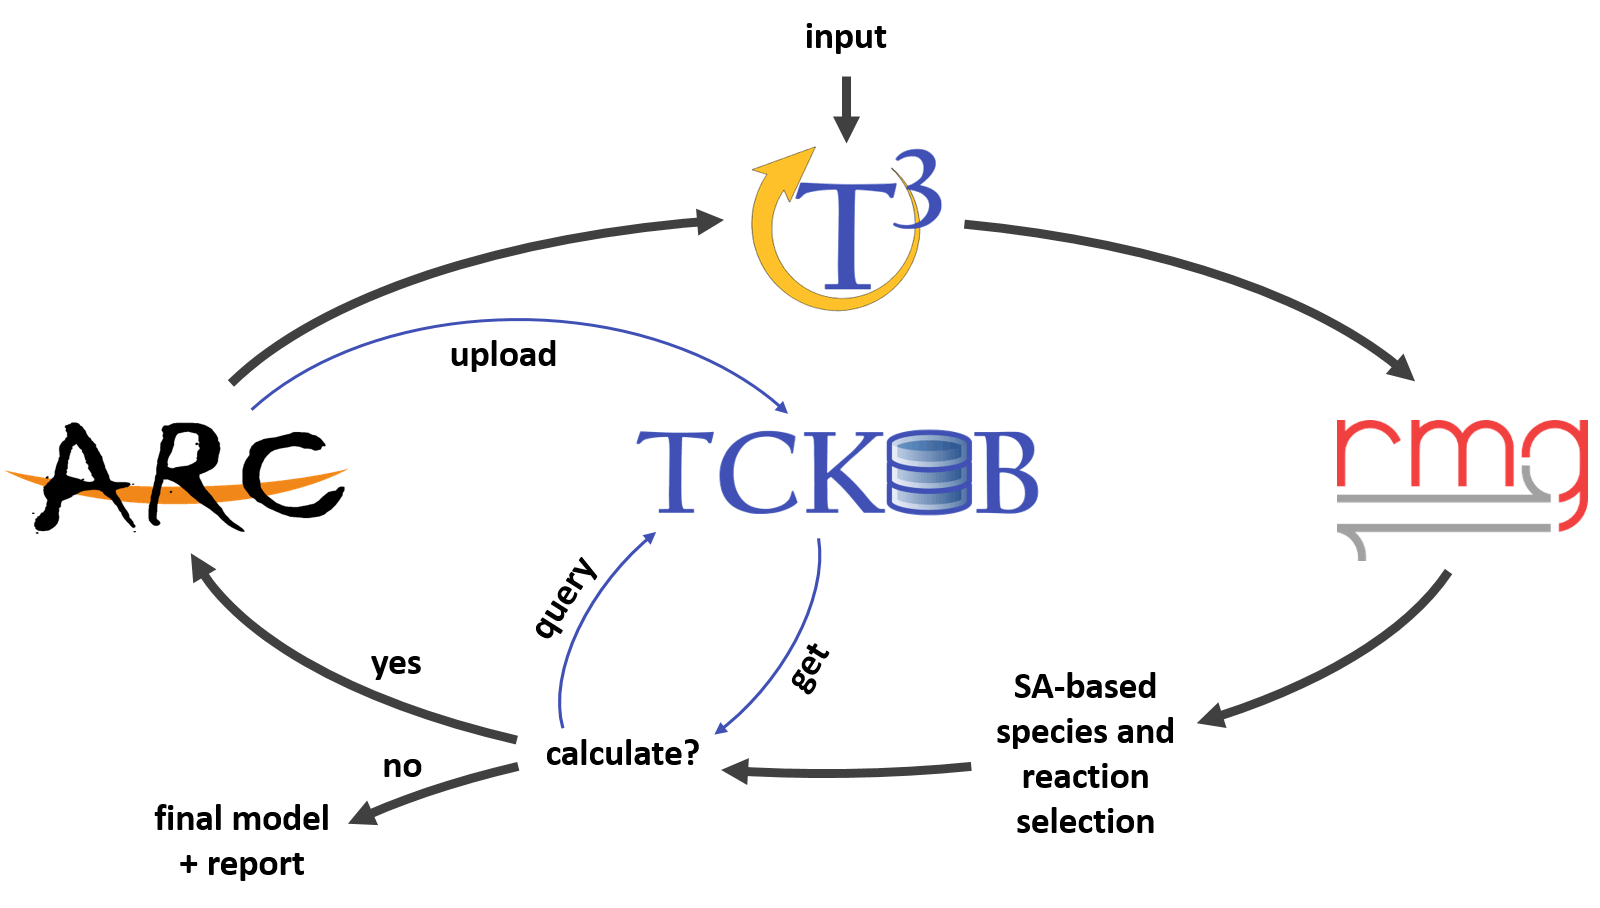
\includegraphics[width=0.9\linewidth]{figures/T3-circle.png}
}

\begin{itemize}
 \item Written in Python 3, released under the MIT License
\end{itemize}

\end{frame}

\begin{frame}{
 \hspace{-5mm}
 
\includegraphics[height=10mm]{figures/Logos/cantera-logo.png}
}

\url{cantera.org}
\hspace{10mm}
\ghinlinelogo\ Cantera/cantera

\vspace{5mm}

\begin{itemize}
 \item ``Cantera is an open-source suite of tools for problems involving chemical kinetics, thermodynamics, and transport processes.''
 \item BSD 3-Clause license
 \item Written in C++; interfaces for programming with Python, C++, Fortran, and Matlab
 \item Built-in classes to represent wide range of gas-phase and surface chemical kinetics, multiple transport models, and reactor classes to consolidate determination of governing equations
 \item Implements Eigen and SUNDIALS libraries for solving equations
 \item Binary distribution on Fedora, RHEL, Ubuntu, Gentoo, FreeBSD, Mac and Windows plus Conda installation
\end{itemize}


\end{frame}

\begin{frame}{ \hspace{-5mm}
 
\includegraphics[height=10mm]{figures/Logos/pyked-logo.png}
 PyKED and ChemKED}
 
 
%\url{rmg.mit.edu}
%\hspace{10mm}
\ghinlinelogo\ pr-omethe-us/PyKED

\vspace{5mm}

\begin{itemize}
 \item ChemKED is a standard human and machine-readable file format for experimental data typical in combustion (\url{github.com/pr-omethe-us/ChemKED-database})
 \item PyKED is a Python interface for validating ChemKED files and implements standard interactions and routines for use with the data (\url{github.com/pr-omethe-us/PyKED})
 \item Written in Python, released under BSD 3-Clause license
\end{itemize}

 
\end{frame}


\begin{frame}{Help wanted}
There is a lot that can be contributed by non-experts in chemistry (actually our biggest deficit):

\begin{itemize}
 \item Cleanup of Conda environments and updating versions of dependencies (e.g. migrating away from \textsc{nosetests}) in \textsc{RMG} and \textsc{ARC}
 \item Developing database for \textsc{TCKDB} with reactions and interfacing to \textsc{T3}
 \item Binary packages and distribution in mainstream repositories on Linux distributions
 \item Overhauling data validating and type-checking in \textsc{PyKED} (old version of \textsc{Cerberus} currently)
\end{itemize}

\end{frame}

\begin{frame}{Q\&A}
 
\end{frame}


\begin{frame}{References}
\printbibliography 
\end{frame}


\end{document}
